The web application, which in this case is Layer X, is the overall web portal that will be used to manage all information for any brewery products.  The web application's sole purpose is to have administrative privileges and more control of the information that is stored in the brewery's database.  Unlike the mobile application, the web portal will allow the user to add, remove, and modify any records of any brewery product that is stored in the database.

\subsection{Manage Inventory}
This section should be a general description of a particular subsystem for the given layer. For most subsystems, an extract of the architectural block diagram with data flows is useful. This should consist of the subsystem being described and those subsystems with which it communicates.

In the Manage Inventory subsystem of the web app layer, the subsystem will allow for information to be managed and stored into the brewery database.  The user will be allowed to add, delete, or modify any brewery records stored in the database by having administrative privileges for easy management of the information stored in the database.

\begin{figure}[h!]
	\centering
 	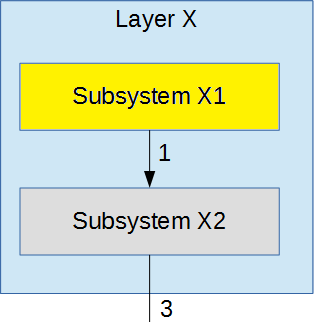
\includegraphics[width=0.60\textwidth]{images/subsystem}
 \caption{Example subsystem description diagram}
\end{figure}

\subsubsection{Assumptions}
Any assumptions made in the definition of the subsystem should be listed and described. Pay particular attention to assumptions concerning interfaces and interactions with other layers.



\subsubsection{Responsibilities}
The Manage Inventory subsystem primary responsibility is for the user to interact with the user interface (UI) that'll be accessible through a web browser in order to manage any and all information stored in the central brewery database.  The user will be able to add, delete, and modify any records that are currently stored and saved on the database.  In addition, the information that'll be made available of any brewery prodcut will include the following:
Name of beer
Style
Date of purchase
Best by date
Format (can, bottle, keg, crowler, growler, etc.)
Location (cabinet, closets, kegerator, etc.)
ID

To further explain the format and location of the brewery, the user will be able to generate a two-dimensional figure to describe the location where the products are stored physically and set the location of the brewery product in the exact row and columns of the two-dimensional figure from the cabinet, closet, kegerator, etc.

\subsubsection{Subsystem Interfaces}
Each of the inputs and outputs for the subsystem are defined here. Create a table with an entry for each labelled interface that connects to this subsystem. For each entry, describe any incoming and outgoing data elements will pass through this interface.

\begin {table}[H]
\caption {Subsystem interfaces} 
\begin{center}
    \begin{tabular}{ | p{1cm} | p{6cm} | p{3cm} | p{3cm} |}
    \hline
    ID & Description & Inputs & Outputs \\ \hline
    \#xx & Description of the interface/bus & \pbox{3cm}{input 1 \\ input 2} & \pbox{3cm}{output 1}  \\ \hline
    \#xx & Description of the interface/bus & \pbox{3cm}{N/A} & \pbox{3cm}{output 1}  \\ \hline
    \end{tabular}
\end{center}
\end{table}

\subsection{Subsystem 2}
Repeat for each subsystem

\subsection{Subsystem 3}
Repeat for each subsystem

